%% Artículo del curso de Biología Computacional (Universidad Nacional de Ingeniería).
%% Plantilla: Oxford University Press (oup-authoring-template, LPPL). Compilar con:
%%   pdflatex main  ->  bibtex main  ->  pdflatex main  ->  pdflatex main
%% (o simplemente subir esta carpeta a Overleaf; ver LEEME.txt)

\documentclass[unnumsec,webpdf,contemporary,large]{oup-authoring-template}

\usepackage[T1]{fontenc}
\usepackage[utf8]{inputenc}
\usepackage[spanish,es-tabla,es-noshorthands]{babel}
\usetikzlibrary{arrows.meta,positioning,calc}

\graphicspath{{Fig/}}
\newcommand{\societylogo}{}
\newcommand{\TODO}[1]{\textcolor{red}{\textbf{[TODO: #1]}}}

\begin{document}

\journaltitle{Biología Computacional --- Informe del curso}
\DOI{--}
\copyrightyear{2026}
\pubyear{2026}
\vol{}
\issue{}
\access{Borrador, octubre de 2026}
\appnotes{Artículo del curso}

\firstpage{1}

\title[Dos proyectos de biología computacional]{Redes de señalización generadas por modelos de lenguaje y clasificación de cáncer con RNA-Seq: dos proyectos de biología computacional}

\author[1,$\ast$]{Pedro Lautaro Quipe Ballesteros}
\author[1]{Omar Quipe Santos}

\address[1]{\orgdiv{Facultad de Ciencias, Carrera de Ciencia de la Computación}, \orgname{Universidad Nacional de Ingeniería}, \orgaddress{\state{Lima}, \country{Perú}}}

\corresp[$\ast$]{Autor de correspondencia. \href{mailto:pedro.quispe.b@uni.pe}{pedro.quispe.b@uni.pe}}

\abstract{Las redes de señalización describen cómo las células transmiten información mediante interacciones de activación e inhibición entre proteínas. Un artículo publicado en eLife en 2026 evaluó si modelos de lenguaje de uso general reconstruyen estas redes a partir de una lista de genes, con 10 réplicas a temperatura 1.0 y medidas de \emph{recall} y precisión frente a redes elaboradas a mano. En el Proyecto~A reproducimos esas métricas con las respuestas guardadas por los autores y las extendemos en la red de hipertrofia cardíaca: con un solo modelo de bajo costo (DeepSeek~V4.1 Flash, sin razonamiento) comparamos la temperatura 1.0 (línea base, 10 réplicas) con la temperatura 0 (3 réplicas), con el mismo prompt y las mismas funciones de evaluación. La reproducción coincidió exactamente con las métricas publicadas en las nueve combinaciones de red y modelo. A temperatura 0 el \emph{recall} aumentó (0.508~$\pm$~0.016 frente a 0.445~$\pm$~0.034; $p=0.003$, exploratorio), la precisión media bajó (0.357~$\pm$~0.104 frente a 0.454~$\pm$~0.059; $p=0.24$) y el F1 casi no cambió. Las respuestas fueron más largas y no reproducibles: ningún par de réplicas resultó idéntico. Las limitaciones son un solo modelo, una sola red y pocas réplicas a temperatura 0. El Proyecto~B (clasificación de cáncer con RNA-Seq) queda como sección reservada.}

\keywords{redes de señalización, modelos de lenguaje, temperatura, reproducibilidad, hipertrofia cardíaca, RNA-Seq}

\otherabstract[Resumen para no especialistas]{Las células de nuestro cuerpo se comunican con cadenas de mensajes químicos: una proteína «avisa» a otra para que se encienda, o le ordena que se apague. Ese conjunto de avisos se llama \emph{red de señalización} y se dibuja como un mapa de flechas: de activación (A enciende a B) o de inhibición (A apaga a B). Armarlos a mano exige leer cientos de artículos, y es lento.

Un grupo de la Universidad de Virginia preguntó si un modelo de lenguaje, es decir, un programa de inteligencia artificial como ChatGPT que escribe texto, puede dibujar ese mapa por sí solo. Le dieron la lista de genes de una red del corazón (la que explica cómo una célula cardíaca crece de más, proceso llamado hipertrofia) y le pidieron las flechas. Compararon sus respuestas con el mapa hecho por expertos con dos medidas: el \emph{recall}, que dice qué parte de las flechas reales encontró, y la precisión, que dice qué parte de las flechas que propuso son reales. Como el programa tiene algo de azar, repitieron cada prueba 10 veces.

Nosotros hicimos dos cosas. Primero, obtuvimos exactamente los mismos números del estudio con las respuestas que sus autores guardaron. Segundo, hicimos un experimento propio con un modelo de bajo costo: ¿qué pasa si le quitamos el azar? Ese azar se controla con la temperatura: con 1.0 el programa varía mucho y con 0 debería responder siempre lo mismo.

Sin azar, el programa propone muchas más flechas: acierta más flechas reales (\emph{recall} de 0.51 frente a 0.44) pero también inventa más (la precisión baja de 0.45 a 0.36), así que el balance casi no cambia. Además, las tres corridas sin azar siguieron siendo distintas entre sí. Y aun con azar, las flechas estables, las que aparecen en las 10 repeticiones, son pocas: 37 de las 191 flechas reales.

Con cautela (un solo modelo, una sola red y pocas repeticiones sin azar), concluimos que estos programas sirven para proponer hipótesis, pero sus respuestas deben contrastarse con expertos. Un segundo proyecto, sobre clasificación de cáncer, se añadirá más adelante.}

\maketitle

%% ---------------------------------------------------------------------------
\section{Introducción general}\label{sec:intro}

La biología computacional usa herramientas matemáticas e informáticas para entender sistemas biológicos. Este informe reúne dos proyectos del curso. En el Proyecto~A estudiamos si los modelos de lenguaje, programas de inteligencia artificial que generan texto, pueden reconstruir redes de señalización celular. En el Proyecto~B, a cargo de otro autor, se clasifican tipos de cáncer a partir de datos de RNA-Seq. Como los dos autores no somos biólogos, definimos cada término técnico la primera vez que aparece, y el Apéndice~A resume los términos principales.

Una célula es la unidad básica de un ser vivo. Su información está guardada en los \emph{genes}, fragmentos de ADN que contienen las instrucciones para fabricar \emph{proteínas}, que son las moléculas que hacen la mayor parte del trabajo celular. Las proteínas no actúan solas: se envían señales unas a otras. Una proteína puede \emph{activar} a otra (aumenta su actividad) o \emph{inhibirla} (la reduce). El conjunto de estas relaciones forma una \emph{red de señalización}, que representamos como un grafo: los \emph{nodos} son proteínas (o grupos de proteínas) y las \emph{flechas} son las activaciones o inhibiciones entre ellas. Estas redes explican, por ejemplo, cómo una célula del corazón responde a una hormona del estrés.

Construir una red de este tipo normalmente exige que expertos lean la literatura científica y registren a mano cada interacción, y luego conviertan la red en un modelo matemático que pueda simularse. Es un trabajo lento. Los \emph{modelos de lenguaje grandes} (LLM, del inglés \emph{large language models}) son programas entrenados con enormes cantidades de texto para predecir la siguiente palabra; esa capacidad les permite responder preguntas, resumir y escribir código~\cite{vaswani2017,brown2020}. Tewari y colaboradores señalan que estos modelos ya han obtenido buenas calificaciones en exámenes de medicina y de derecho, lo que plantea la pregunta de si pueden ayudar a reconstruir redes biológicas a partir de lo que han «leído»; ellos publicaron en 2026 una evaluación sistemática de esta idea~\cite{tewari2026}, que es la base del Proyecto~A.

El resto del informe se organiza así: la Sección~\ref{sec:A} presenta el Proyecto~A (contexto, métodos, resultados y discusión), la Sección~\ref{sec:B} está reservada para el Proyecto~B, y los apéndices contienen un glosario.

%% ---------------------------------------------------------------------------
\section{Proyecto A: redes bioquímicas generadas por modelos de lenguaje}\label{sec:A}

\subsection{Contexto y pregunta de investigación}\label{sec:A:contexto}

Tewari y colaboradores~\cite{tewari2026} entregaron a un LLM la lista de genes de una red de señalización y le pidieron las interacciones entre ellos (activa o inhibe). Luego compararon la red generada con una \emph{red de referencia} elaborada a mano por expertos y validada con experimentos de la literatura, que en su artículo se llama \emph{ground truth}. Evaluaron tres redes cardíacas: hipertrofia~\cite{ryall2012}, activación de fibroblastos~\cite{zeigler2016} y mecanoseñalización~\cite{tan2017}, con tres LLM (GPT-5.2 Pro, Gemini~3 Pro y Claude Opus 4.6). Como el LLM tiene un componente aleatorio, cada consulta se repitió 10 veces (\emph{réplicas}). El artículo también simula perturbaciones con las redes generadas (con el marco de modelado lógico Netflux~\cite{clark2025}) y estudia la red metabólica central de \emph{Escherichia coli}; nosotros no reprodujimos esas partes.

Dos medidas resumen el desempeño. El \emph{recall} (en el repositorio, «sensibilidad») es la fracción de las flechas de la red de referencia que el LLM encontró. La \emph{precisión} es la fracción de las flechas que el LLM propuso que existen en la red de referencia. Un ejemplo sencillo: si la red de referencia tiene 10 flechas y el LLM propone 8, de las cuales 4 son reales, el \emph{recall} es $4/10=0.4$ y la precisión es $4/8=0.5$. Los autores del paper advierten que una flecha propuesta que no está en la red de referencia no necesariamente es falsa, pues podría ser una interacción real que los curadores no incluyeron~\cite{tewari2026}; aun así, la tratan como «falso positivo» para calcular métricas, y nosotros hacemos lo mismo.

Entre las respuestas a los revisores, los propios autores señalan que la frecuencia con que una flecha aparece entre las réplicas, que usan como indicador de confianza, depende mucho del parámetro de \emph{temperatura} de los LLM~\cite{tewari2026}. La temperatura controla cuánto azar usa el modelo al elegir cada palabra: con valores altos (1.0 por defecto en muchas interfaces) las respuestas varían más, y con 0 el modelo debería elegir siempre la opción más probable. Esa observación motiva nuestra pregunta:

\begin{quote}
\emph{En la red de hipertrofia, ¿cambia el \emph{recall} y la precisión cuando se baja la temperatura de 1.0 a 0, usando un único modelo gratuito o de bajo costo?}
\end{quote}

Nuestra línea base es nuestro propio modelo a temperatura 1.0, que es el valor que usó el paper. Los resultados del paper se muestran solo como contexto: son otros modelos, de otros tamaños y proveedores, y no podemos compararlos directamente con el nuestro.

\subsection{Métodos}\label{sec:A:metodos}

\subsubsection{Red de referencia}

Usamos la red de hipertrofia cardíaca~\cite{ryall2012}: el proceso por el cual una célula del corazón (\emph{cardiomiocito}) aumenta de tamaño en respuesta a estímulos como la angiotensina~II o la fenilefrina. El archivo del repositorio contiene 106 nodos y 193 reglas; algunas reglas son de tipo \emph{AND} (una flecha solo ocurre si dos proteínas coinciden), y al separarlas en pares origen-destino quedan 191 conexiones dirigidas distintas. Cada nodo tiene asociados uno o más genes, por lo que la lista que recibe el LLM tiene 225 genes. El prompt también recibe un valor máximo de conexiones por nodo, calculado como en el repositorio a partir de la propia red de referencia (14 para hipertrofia); es decir, el LLM recibe una pista sobre cuántas conexiones esperar, igual que en el paper.

\subsubsection{Reproducción de las métricas del paper}

Clonamos el repositorio público de los autores~\cite{repo_saucerman} (licencia MIT; no modificamos ninguno de sus archivos). Con las 10 respuestas guardadas por cada combinación de red y LLM (90 archivos), recalculamos el \emph{recall} y la precisión con las funciones del repositorio. Como esas métricas están dentro de un cuaderno de Jupyter y no son importables, copiamos su lógica en un módulo propio sin cambiar el criterio. Comparamos nuestros resultados con la tabla de resumen y con las tablas de conteos incluidas en el repositorio.

\subsubsection{Experimento: efecto de la temperatura}

\paragraph{Modelo.} Usamos DeepSeek~V4.1 Flash (nombre en la API: \texttt{deepseek-flash}~\cite{deepseek_models}) a través de su API, un servicio que permite enviar instrucciones a un modelo por internet. Elegimos un modelo de bajo costo porque no teníamos presupuesto para los modelos del paper. Nuestro plan inicial, Llama~3.3~70B en un plan gratuito, no fue posible porque el proveedor ya había retirado ese modelo. DeepSeek activa por defecto un modo de razonamiento en el que la temperatura \emph{no tiene efecto}~\cite{deepseek_thinking}; por eso lo desactivamos en cada llamada, y comprobamos que las respuestas no incluyeran razonamiento (0 de 156 llamadas lo incluyeron).

\paragraph{Prompt y procedimiento.} Los mensajes de usuario son idénticos a los del repositorio (comparamos el texto por programa): primero la lista de genes; luego se pide, para los primeros 20 genes, más de 0 y menos de 14 interacciones directas respaldadas por la literatura en formato JSON, cada una con \texttt{source\_node}, \texttt{target\_node} y \texttt{action} (\texttt{stimulation} o \texttt{inhibition}); y después se repite «That looks great! Please do the same operation for the next $N$ nodes!» hasta cubrir los 225 genes (Figura~\ref{fig:esquema}). JSON es un formato de texto estructurado para intercambiar datos. Son 12 llamadas por réplica, y cada llamada incluye toda la conversación anterior, como en el paper. Un \emph{token} es la unidad de texto que procesa el modelo (aproximadamente una sílaba o una palabra corta); fijamos 4000 tokens como máximo de salida por llamada, el valor por defecto del repositorio.

\paragraph{Condiciones.} Temperatura 1.0 (línea base) con 10 réplicas y temperatura 0 con 3 réplicas, en total 13 réplicas y 156 llamadas. Las réplicas se intercalaron en el tiempo (1.0, 0, 1.0, 0, \ldots) y se ejecutaron el 25 de octubre de 2026. Cada respuesta se guardó en disco apenas llegó y se registró su estado: correcta, vacía, mal formada, cortada por límite de tokens o rechazada. Cada llamada fallida se reintentaba hasta completar 3 intentos.

\paragraph{Diferencias con el protocolo del paper.} La Tabla~\ref{tab:diferencias} las resume. Lo más importante: (i) el paper indica un máximo de salida de 10\,000 tokens en su texto, mientras que nosotros partimos del valor por defecto del repositorio, 4000; (ii) DeepSeek no puede forzar el esquema de la respuesta, solo garantizar que sea JSON válido, así que añadimos un mensaje de sistema que describe el formato y validamos cada respuesta con las mismas clases del repositorio; (iii) si una respuesta se cortaba por el límite de tokens, el reintento usaba un máximo de 16\,000 tokens, por encima de los 10\,000 del paper, de modo que ninguna respuesta final quedó cortada.

\begin{table*}[t]
\caption{Diferencias entre nuestro experimento y el protocolo del paper~\cite{tewari2026}.\label{tab:diferencias}}
\begin{tabular*}{\textwidth}{@{\extracolsep\fill}p{3.3cm}p{6.2cm}p{6.2cm}@{}}
\toprule
Aspecto & Paper & Nuestro experimento \\
\midrule
Modelos & GPT-5.2 Pro, Gemini 3 Pro, Claude Opus 4.6 & DeepSeek V4.1 Flash (uno solo) \\
Temperatura & 1.0 & 1.0 (línea base) y 0 \\
Réplicas por condición & 10 & 10 a temperatura 1.0 y 3 a temperatura 0 \\
Redes & Hipertrofia, fibroblasto y mecanoseñalización & Solo hipertrofia \\
Máximo de salida & 10\,000 tokens (según el texto del paper) & 4000 (por defecto del repositorio); 16\,000 en los reintentos de respuestas cortadas \\
Formato de salida & Salida estructurada con esquema forzado & Modo JSON, mensaje de sistema y validación con el mismo esquema \\
Razonamiento & Modelos de razonamiento & Desactivado \\
Instrucciones (prompt) & Las descritas arriba & Idénticas en los mensajes de usuario \\
\botrule
\end{tabular*}
\end{table*}

\begin{figure*}[t]
\centering
\begin{tikzpicture}[
  font=\small, >=Stealth,
  caja/.style={draw, rounded corners=3pt, align=center, minimum height=1.3cm, text width=3.5cm, fill=black!4},
  nota/.style={font=\footnotesize, align=center, text=black!70}]
\node[caja] (a) {Lista de 225 genes\\ de la red de hipertrofia};
\node[caja, right=0.9cm of a] (b) {Modelo de lenguaje\\ 12 llamadas, lotes de 20 genes,\\ con el historial de la conversación};
\node[caja, right=0.9cm of b] (c) {Flechas propuestas\\ (origen, destino,\\ activa o inhibe) en JSON};
\node[caja, right=0.9cm of c] (d) {Comparación con la red\\ hecha a mano:\\ \emph{recall} y precisión};
\draw[->] (a)--(b); \draw[->] (b)--(c); \draw[->] (c)--(d);
\node[nota, below=0.5cm of b] (r) {Se repite: 10 réplicas a temperatura 1.0 y 3 réplicas a temperatura 0};
\draw[->, black!50] (r.north) -- (b.south);
\end{tikzpicture}
\caption{Esquema del procedimiento del Proyecto~A. El mismo procedimiento se aplicó a las dos temperaturas; solo cambió el parámetro de temperatura.\label{fig:esquema}}
\end{figure*}

\subsubsection{Evaluación y estadística}

Las respuestas del LLM nombran genes; los traducimos a los nodos de la red (comparando los nombres sin distinguir mayúsculas). Construimos una matriz de $106\times106$ con 1 si hay estimulación, $-1$ si hay inhibición y 0 si no hay flecha, para la red de referencia y para cada réplica. Una flecha es acierto (\emph{verdadero positivo}, TP) solo si coinciden origen, destino \emph{y signo}. Una flecha propuesta que no está en la referencia, o que está con el signo contrario, es un \emph{falso positivo} (FP); una flecha de la referencia que el LLM no propuso es un \emph{falso negativo} (FN). Entonces
\begin{gather}
\text{recall}=\frac{TP}{TP+FN},\qquad
\text{precisión}=\frac{TP}{TP+FP},\nonumber\\
F_1=\frac{2\cdot\text{precisión}\cdot\text{recall}}{\text{precisión}+\text{recall}}.
\label{eq:metricas}
\end{gather}
El $F_1$ es un promedio de las dos medidas que solo es alto si ambas lo son. Como verificación cruzada, también contamos los TP con la función \texttt{compare\_connections} del repositorio.

Para cada temperatura calculamos la media y la desviación estándar muestral (con $n-1$) entre réplicas, y comparamos las dos temperaturas con la prueba $t$ de Welch~\cite{welch1947}, que no supone varianzas iguales. Dado que hay solo 3 réplicas a temperatura 0 y se hicieron 3 pruebas, estos valores $p$ son \emph{exploratorios}. Para medir el parecido entre dos réplicas usamos el índice de Jaccard~\cite{jaccard1912}, $|A\cap B|/|A\cup B|$, donde $A$ y $B$ son los conjuntos de interacciones propuestas (1 si son idénticas, 0 si no comparten ninguna). Usamos Python con NumPy, pandas, SciPy y Matplotlib~\cite{numpy2020,pandas2010,scipy2020,hunter2007}.

\subsection{Resultados}\label{sec:A:resultados}

\subsubsection{La reproducción coincide con el paper}

Con las respuestas guardadas recalculamos el \emph{recall} y la precisión de las tres redes y los tres LLM (Tabla~\ref{tab:repro} y Figura~\ref{fig:paper}). Los valores medios coinciden \emph{exactamente} (diferencia 0) con la tabla de resumen del repositorio en las 9 combinaciones. Los extremos que el artículo reporta en el texto para la hipertrofia (37.70--63.87\,\%) corresponden a 72 y 122 flechas halladas de 191, es decir, el mínimo y el máximo entre réplicas de los conteos guardados; lo mismo ocurre con los extremos del fibroblasto y de la mecanoseñalización.

Hay una discrepancia menor en mecanoseñalización: la tabla de conteos guardada difiere de la que genera el código actual del repositorio en una flecha por réplica ($\text{AngII}\to\text{AT1R}$; 10 a 11 celdas por LLM). La causa que identificamos es que el código busca un nodo llamado \texttt{AGT} para duplicar la flecha, pero en esa red el segundo nodo con ese gen se llama \texttt{Ao}. Esto no afecta las métricas formales, que sí coinciden, ni nuestro experimento, que usa solo la hipertrofia. En hipertrofia y fibroblasto las tablas coinciden por completo.

En el contexto del paper (Tabla~\ref{tab:repro}), Claude y GPT encuentran más flechas (mayor \emph{recall}) pero proponen muchas que no están en la referencia (menor precisión), mientras que Gemini es más conservador: encuentra menos, pero acierta más de lo que propone.

\begin{table*}[t]
\caption{Reproducción de las métricas del paper con las respuestas guardadas (temperatura 1.0, 10 réplicas por modelo y red). Se muestra la media $\pm$ desviación estándar. TP y FP son promedios por réplica. En las 9 combinaciones, los valores coinciden con el resumen incluido en el repositorio.\label{tab:repro}}
\begin{tabular*}{\textwidth}{@{\extracolsep\fill}llcccc@{}}
\toprule
Red & Modelo & TP & FP & \emph{Recall} & Precisión \\
\midrule
Hipertrofia & Claude Opus 4.6 & 119.0 & 103.0 & 0.632 $\pm$ 0.013 & 0.537 $\pm$ 0.025 \\
 & GPT-5.2 Pro & 107.5 & 124.7 & 0.566 $\pm$ 0.021 & 0.464 $\pm$ 0.029 \\
 & Gemini 3 Pro & 74.5 & 24.9 & 0.390 $\pm$ 0.017 & 0.751 $\pm$ 0.034 \\
\midrule
Fibroblasto & Claude Opus 4.6 & 94.2 & 201.6 & 0.591 $\pm$ 0.014 & 0.319 $\pm$ 0.013 \\
 & GPT-5.2 Pro & 72.1 & 141.4 & 0.452 $\pm$ 0.033 & 0.342 $\pm$ 0.035 \\
 & Gemini 3 Pro & 45.5 & 17.9 & 0.281 $\pm$ 0.020 & 0.717 $\pm$ 0.032 \\
\midrule
Mecanoseñalización & Claude Opus 4.6 & 106.4 & 215.8 & 0.642 $\pm$ 0.016 & 0.332 $\pm$ 0.021 \\
 & GPT-5.2 Pro & 81.5 & 173.7 & 0.482 $\pm$ 0.041 & 0.330 $\pm$ 0.057 \\
 & Gemini 3 Pro & 56.2 & 21.6 & 0.328 $\pm$ 0.041 & 0.729 $\pm$ 0.047 \\
\botrule
\end{tabular*}
\end{table*}

\begin{figure*}[t]
\centering
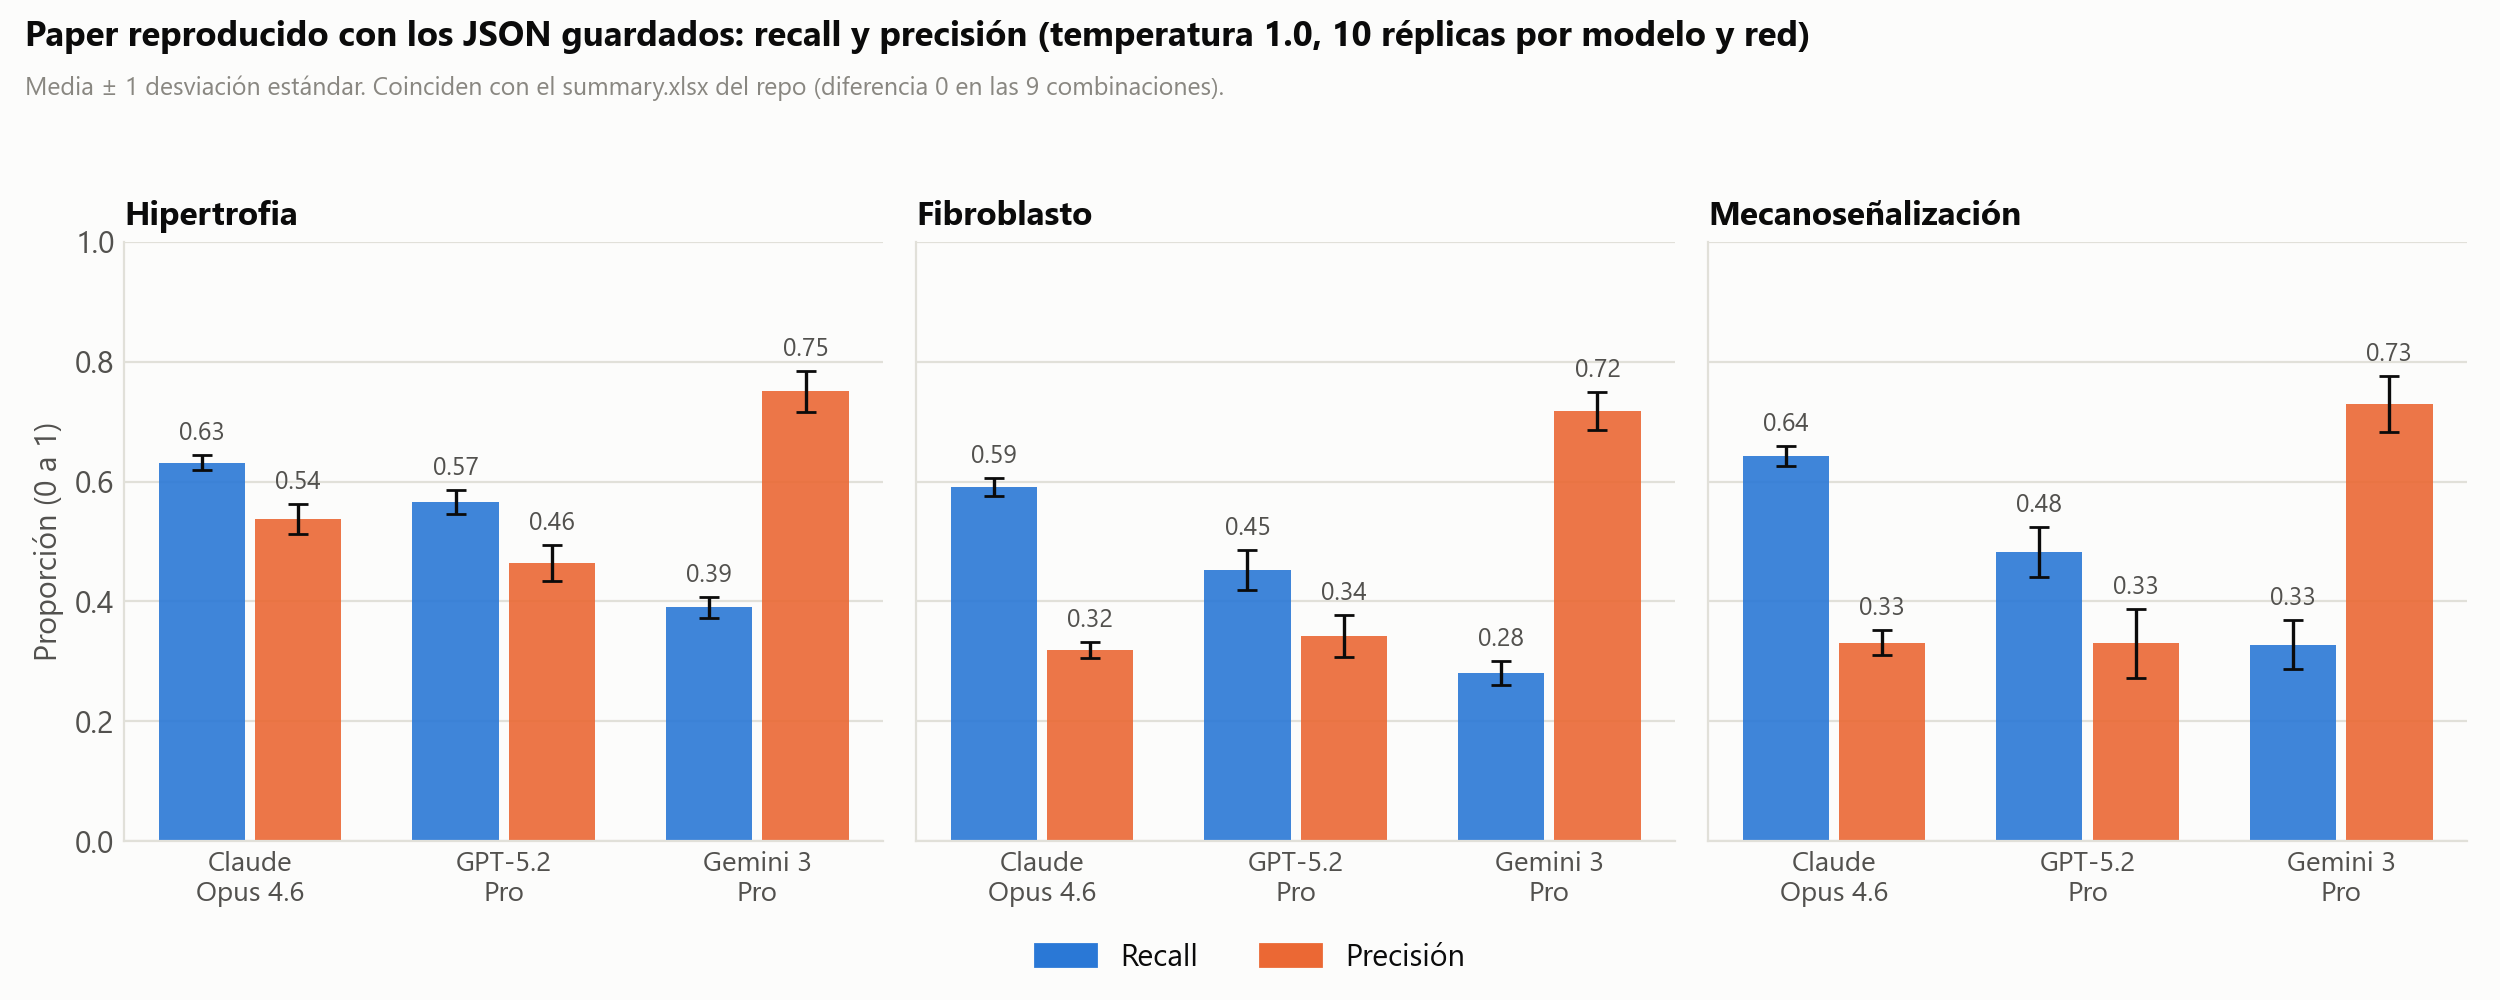
\includegraphics[width=\textwidth]{fig_metricas_paper.png}
\caption{Métricas del paper reproducidas con las respuestas guardadas por sus autores: \emph{recall} (azul) y precisión (naranja), media $\pm$ 1 desviación estándar, a temperatura 1.0 con 10 réplicas por modelo y red. Los modelos son los del paper, no el nuestro.\label{fig:paper}}
\end{figure*}

\subsubsection{Efecto de la temperatura en el \emph{recall} y la precisión}

Completamos las 13 réplicas (156 llamadas). La Tabla~\ref{tab:temperatura} y la Figura~\ref{fig:temperatura} resumen el resultado. A temperatura 1.0 (línea base), el \emph{recall} medio fue 0.445 y la precisión media 0.454. A temperatura 0, el \emph{recall} subió a 0.508 y la precisión bajó a 0.357. La diferencia de \emph{recall} es clara (prueba de Welch exploratoria, $p=0.003$; con una corrección de Bonferroni por las 3 pruebas, $p\approx0.008$); la de precisión no es concluyente ($p=0.24$) porque la variación entre las 3 réplicas a temperatura 0 es grande (0.26--0.47). El $F_1$ no cambió de forma apreciable (0.446 frente a 0.412; $p=0.47$).

Esto se relaciona con el tamaño de las respuestas. A temperatura 0, el modelo escribió en promedio 1098 interacciones por réplica (903--1269) frente a 479 (301--679) a temperatura 1.0, y la cantidad de flechas únicas entre nodos de la red (tras traducir los genes a nodos) pasó de 190 a 287. Más flechas propuestas significan más aciertos (TP: 96.3 frente a 84.3), pero también muchos más falsos positivos (191.0 frente a 105.6). Los falsos negativos casi no cambiaron (93.3 frente a 105.2).

\begin{table}[t]
\caption{Resultados por temperatura (red de hipertrofia, DeepSeek V4.1 Flash). Media $\pm$ desviación estándar entre réplicas; entre paréntesis, el mínimo y el máximo. Valores $p$ de la prueba $t$ de Welch (exploratoria).\label{tab:temperatura}}
\begin{tabular*}{\columnwidth}{@{\extracolsep\fill}lcc@{}}
\toprule
 & Temperatura 1.0 & Temperatura 0 \\
 & ($n=10$) & ($n=3$) \\
\midrule
\emph{Recall} & 0.445 $\pm$ 0.034 & 0.508 $\pm$ 0.016 \\
Precisión & 0.454 $\pm$ 0.059 & 0.357 $\pm$ 0.104 \\
$F_1$ & 0.446 $\pm$ 0.028 & 0.412 $\pm$ 0.066 \\
TP & 84.3 & 96.3 \\
FP & 105.6 & 191.0 \\
FN & 105.2 & 93.3 \\
Flechas únicas entre nodos de la red & 189.9 & 287.3 \\
Interacciones en bruto & 479 (301--679) & 1098 (903--1269) \\
\midrule
$p$ (\emph{recall}) & \multicolumn{2}{c}{0.003} \\
$p$ (precisión) & \multicolumn{2}{c}{0.24} \\
$p$ ($F_1$) & \multicolumn{2}{c}{0.47} \\
\botrule
\end{tabular*}
\end{table}

\begin{figure}[t]
\centering
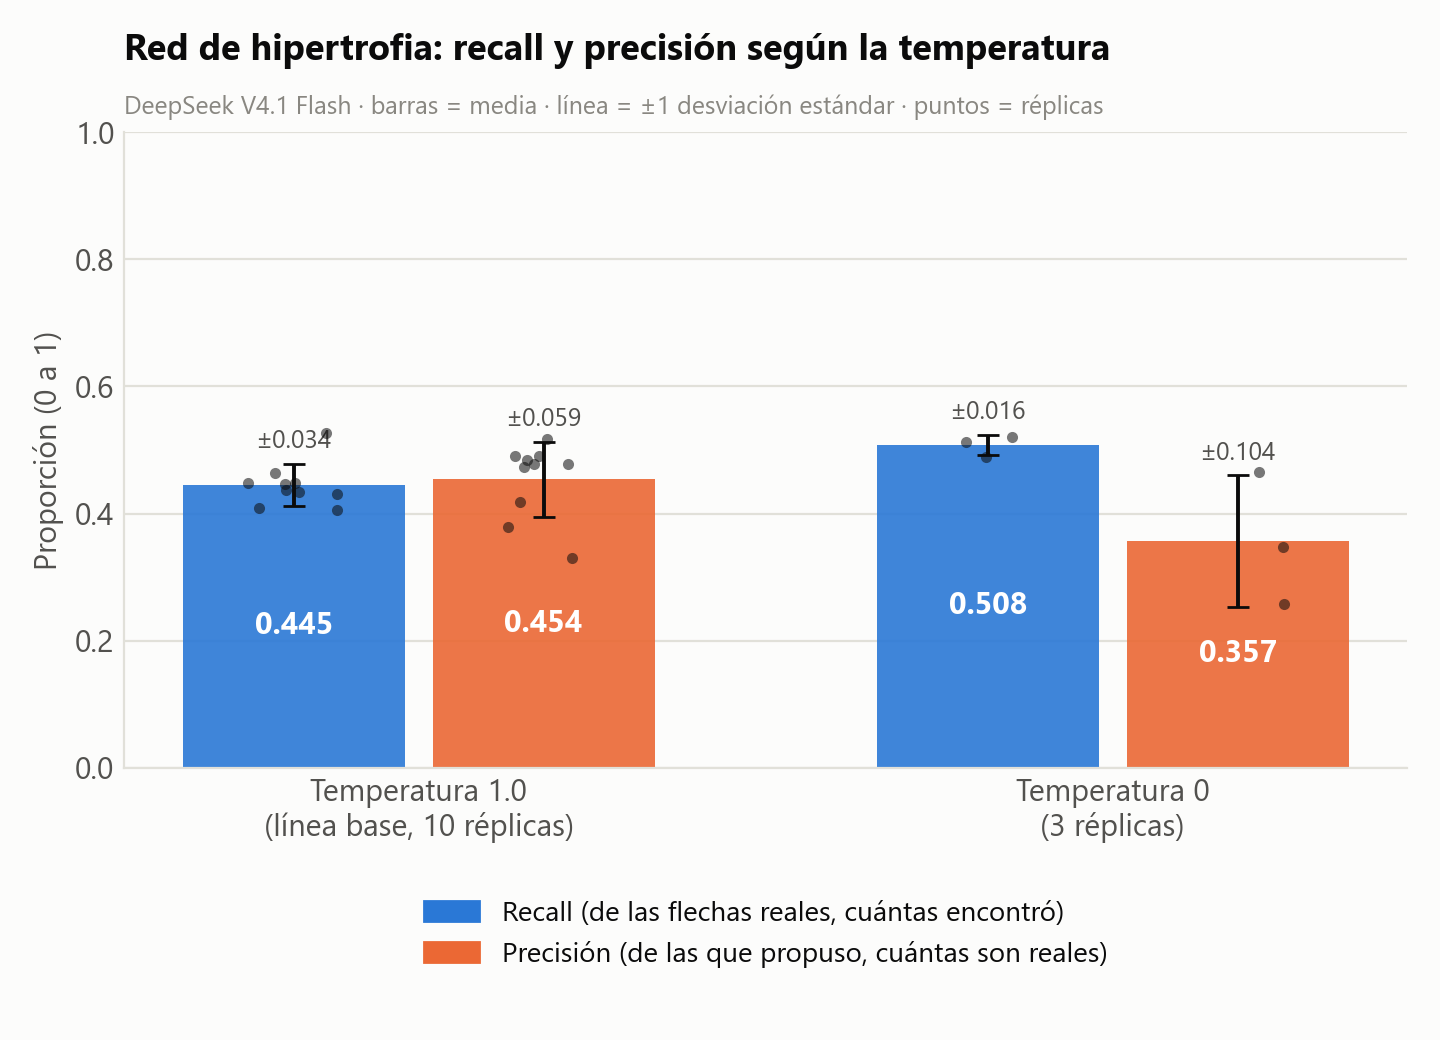
\includegraphics[width=\columnwidth]{fig_recall_precision_temperatura.png}
\caption{\emph{Recall} (azul) y precisión (naranja) por temperatura en la red de hipertrofia. Las barras son la media, las líneas son $\pm$1 desviación estándar y los puntos son las réplicas individuales.\label{fig:temperatura}}
\end{figure}

\subsubsection{Estabilidad de las flechas entre réplicas}

Entre las 10 réplicas a temperatura 1.0, se propusieron 525 flechas distintas al menos una vez: 130 de las 191 flechas reales y 395 que no están en la red; 61 flechas reales no fueron propuestas por ninguna réplica (Figura~\ref{fig:frecuencias}, izquierda). Solo 43 flechas aparecen en las 10 réplicas (37 son reales), mientras que 204 aparecen en una sola réplica (solo 21 son reales). La frecuencia es informativa: entre las flechas que aparecen en 8 o más réplicas, 68 de 94 (72\,\%) son reales; entre las que aparecen en una sola, 21 de 204 (10\,\%). A temperatura 0 (3 réplicas), 147 flechas aparecieron en las tres réplicas (82 reales), 241 en una sola (21 reales) y 77 flechas reales nunca se propusieron (Figura~\ref{fig:frecuencias}, derecha).

\begin{figure*}[t]
\centering
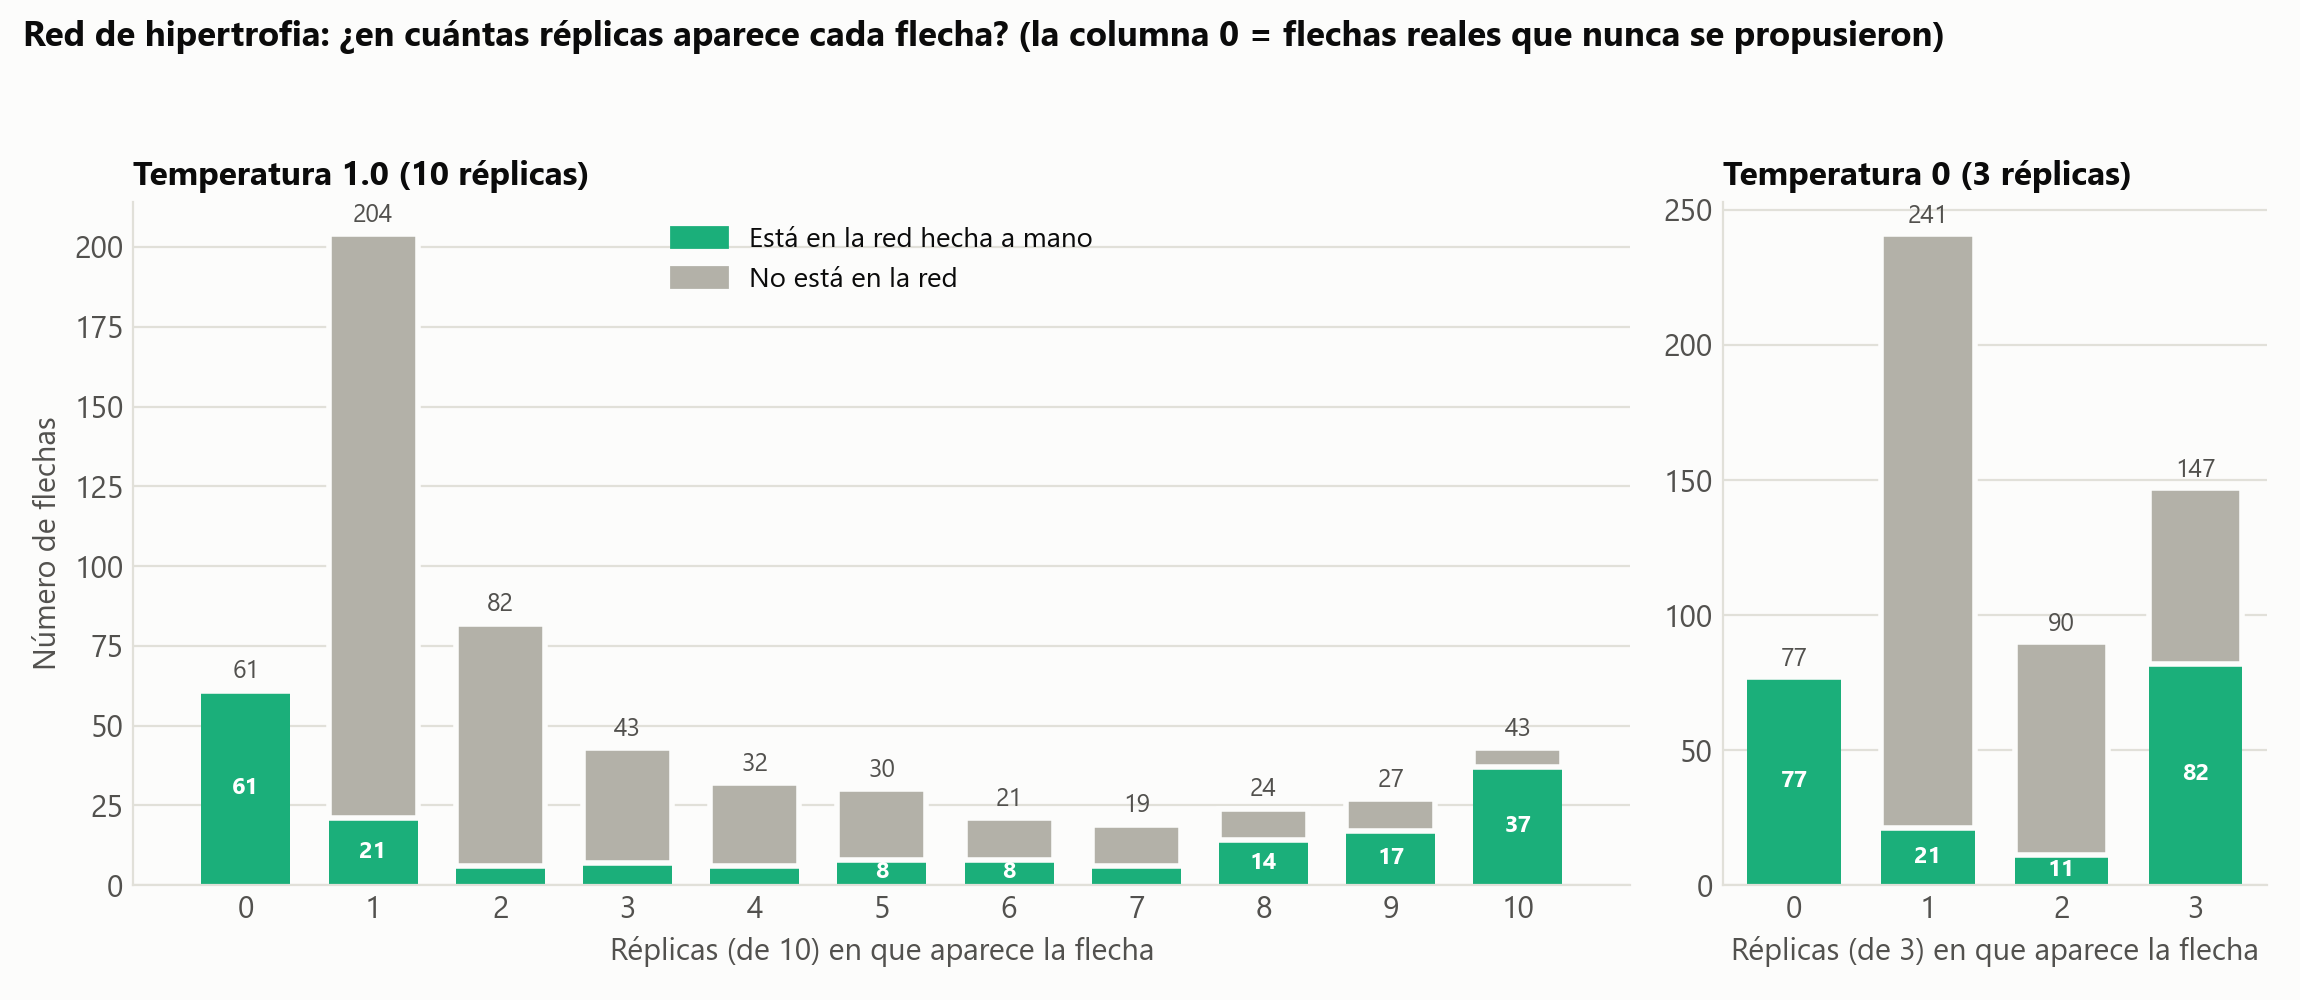
\includegraphics[width=\textwidth]{fig_frecuencia_flechas.png}
\caption{Número de flechas según en cuántas réplicas aparecen, a temperatura 1.0 (10 réplicas, izquierda) y temperatura 0 (3 réplicas, derecha). Verde: la flecha está en la red hecha a mano; gris: no está. La columna 0 contiene las flechas reales que ninguna réplica propuso.\label{fig:frecuencias}}
\end{figure*}

\subsubsection{La temperatura 0 no fue reproducible}

Ningún par de réplicas a temperatura 0 salió idéntico (0 de 3 pares, tanto en el orden como en el contenido). El índice de Jaccard entre pares fue 0.41, 0.46 y 0.49 (media 0.45), algo mayor que a temperatura 1.0 (media 0.36; rango 0.25--0.56; 45 pares), pero lejos de 1. Esto ocurre incluso en la primera llamada de cada réplica, que recibe exactamente la misma entrada: a temperatura 0 devolvió 111, 149 y 111 interacciones (Jaccard medio 0.50), y a temperatura 1.0 devolvió entre 25 y 82 (Jaccard medio 0.32). Es decir, bajar la temperatura a 0 no basta para obtener resultados repetibles con este servicio, en línea con estudios previos que reportan no determinismo con configuraciones «deterministas»~\cite{atil2024,ouyang2023}.

\subsubsection{Calidad de las respuestas}

De 160 respuestas, 156 fueron correctas (Tabla~\ref{tab:calidad}). Hubo 4 respuestas cortadas por llegar al máximo de 4000 tokens, todas a temperatura 0 (4 de 40 respuestas, un 10\,\%); cada una se reintentó con 16\,000 tokens y quedó completa. No hubo respuestas vacías, mal formadas por otra causa ni rechazadas, ni errores de la API, ni interacciones descartadas por no cumplir el formato, ni razonamiento en la respuesta. El costo total fue de unos 0.29 dólares (1.64 millones de tokens de entrada y 0.22 millones de salida; sin contar una corrida inicial interrumpida). Cada réplica tardó entre 36 y 63 s a temperatura 1.0 y entre 91 y 130 s a temperatura 0.

\begin{table}[t]
\caption{Estado de las respuestas de la API por temperatura. «Cortada» es una respuesta que llegó al máximo de 4000 tokens y dejó el JSON incompleto.\label{tab:calidad}}
\begin{tabular*}{\columnwidth}{@{\extracolsep\fill}lcc@{}}
\toprule
 & Temp. 1.0 & Temp. 0 \\
\midrule
Respuestas totales & 120 & 40 \\
Correctas & 120 & 36 \\
Cortadas (límite de tokens) & 0 & 4 \\
Mal formadas (otra causa) & 0 & 0 \\
Vacías o sin contenido & 0 & 0 \\
Rechazadas & 0 & 0 \\
Tokens de entrada / salida (miles) & 985 / 129 & 656 / 89 \\
\botrule
\end{tabular*}
\end{table}

\subsection{Discusión}\label{sec:A:discusion}

\paragraph{Qué encontramos.} Con este modelo, bajar la temperatura a 0 no mejora la reconstrucción de la red: cambia el equilibrio entre cubrir más flechas reales y proponer más flechas que no están en la referencia. El \emph{recall} sube (más cobertura) y la precisión tiende a bajar (más falsos positivos), mientras que el $F_1$, que combina ambas, queda prácticamente igual. Por eso interpretamos el efecto como un desplazamiento a lo largo de un mismo compromiso entre cobertura y precisión, causado en gran parte por listas más largas, y no como una mejora de calidad. Una explicación posible, que no pusimos a prueba, es que sin azar el modelo enumera de manera sistemática todas las interacciones plausibles de cada gen (por ejemplo, entre todos los miembros de una familia de genes), mientras que con azar da respuestas más cortas y variadas.

\paragraph{Reproducibilidad.} La temperatura 0 no sustituye a las réplicas: con este servicio las respuestas siguen siendo distintas entre sí. Además, el comportamiento a temperatura 0 fue más ruidoso de lo esperado en la precisión (0.26--0.47 entre solo 3 réplicas). La frecuencia con que aparece una flecha entre réplicas es un indicador razonable de confianza (72\,\% de las flechas que aparecen en 8 o más réplicas son reales, frente a 10\,\% de las que aparecen una vez), lo que concuerda con la observación de los autores del paper de que esa frecuencia depende de la temperatura~\cite{tewari2026}. Nuestros datos muestran que la distribución de frecuencias cambia mucho con la temperatura (Figura~\ref{fig:frecuencias}).

\paragraph{Contexto con el paper.} Nuestra línea base (\emph{recall} 0.445 y precisión 0.454) queda dentro del rango de recall de los modelos del paper en hipertrofia (0.390--0.632) y cerca de GPT-5.2 Pro en precisión (0.464), pero insistimos en que no es una comparación directa: los modelos, el tamaño, el formato de salida y el tope de tokens son distintos (Tabla~\ref{tab:diferencias}).

\paragraph{Limitaciones.}
\begin{itemize}
\item \textbf{Un solo modelo, una sola red.} No sabemos si el patrón se repite en otros modelos o en las redes de fibroblasto y mecanoseñalización.
\item \textbf{Pocas réplicas a temperatura 0} ($n=3$). La comparación de la precisión no es concluyente y los valores $p$ son exploratorios.
\item \textbf{Tope de tokens.} Partimos de 4000 tokens (valor por defecto del repositorio) mientras el texto del paper indica 10\,000. Las 4 respuestas que se cortaron (todas a temperatura 0) se regeneraron con 16\,000, por encima del tope del paper, así que ninguna respuesta final quedó truncada. Pero las respuestas regeneradas son muestras nuevas, no la misma respuesta completada, y su efecto sobre los promedios no se midió; con 4 de 156 llamadas creemos que es pequeño.
\item \textbf{Formato de salida.} El modo JSON no fuerza el esquema; en la práctica el modelo lo respetó (0 interacciones descartadas), pero es una diferencia de método con los modelos del paper.
\item \textbf{La referencia no es perfecta.} Una flecha propuesta que no está en la red de referencia puede ser real. Esto afecta sobre todo a la precisión a temperatura 0, donde hay muchas más flechas propuestas. No revisamos la literatura para decidir cuáles son reales.
\item \textbf{Pista en el prompt.} El valor de conexiones máximas viene de la red de referencia, igual que en el paper.
\item \textbf{Alcance.} No reprodujimos la simulación de perturbaciones ni la red metabólica de \emph{E.~coli} del artículo original.
\end{itemize}

\paragraph{Trabajo futuro.} Repetir el experimento con otros modelos y con las otras dos redes; usar más réplicas a temperatura 0 y el tope de 10\,000 tokens; y revisar manualmente una muestra de las flechas «falsas» para estimar cuántas son interacciones reales.

%% ---------------------------------------------------------------------------
\section{Proyecto B: clasificación de cáncer con RNA-Seq}\label{sec:B}

\TODO{Sección reservada para el proyecto de Omar Quipe Santos (aún no realizado). Aquí irán: contexto (qué es RNA-Seq y qué es clasificar tipos de cáncer), métodos, resultados y discusión, con el mismo nivel de definición de términos que el Proyecto~A.}

\subsection{Métodos}
\vspace{3.5cm}

\subsection{Resultados}
\vspace{3.5cm}

\subsection{Discusión}
\vspace{3.5cm}

%% ---------------------------------------------------------------------------
\section{Disponibilidad de datos y código}
El código y las respuestas guardadas del estudio original están en el repositorio de los autores~\cite{repo_saucerman} (licencia MIT), que debe citarse al reutilizarlo. Nuestro código propio (módulo de evaluación, ejecución del experimento, cuadernos de análisis), las 156 respuestas crudas del modelo, los archivos CSV de resultados, las figuras y el código fuente de este artículo están en un repositorio público de GitHub: \TODO{poner aquí la URL del repositorio}.

\section{Conflicto de intereses}
Los autores declaran que no tienen conflictos de intereses.

\bibliographystyle{oup-plain}
\bibliography{referencias}

%% ---------------------------------------------------------------------------
\begin{appendices}

\section{Glosario}\label{app:glosario}

\begin{unlist}
\item \textbf{Activación e inhibición.} Una proteína activa a otra si aumenta su actividad, y la inhibe si la reduce.
\item \textbf{API.} Servicio que permite enviar instrucciones a un modelo de lenguaje por internet y recibir su respuesta.
\item \textbf{Cardiomiocito e hipertrofia.} Un cardiomiocito es una célula del músculo del corazón; la hipertrofia es el aumento de su tamaño.
\item \textbf{Falso negativo, falso positivo, verdadero positivo.} Flecha real no propuesta (FN); flecha propuesta que no está en la referencia o tiene el signo contrario (FP); flecha propuesta que sí está en la referencia, con el mismo signo (TP).
\item \textbf{Gen y proteína.} El gen es un fragmento de ADN con instrucciones; la proteína es la molécula que se fabrica con ellas.
\item \textbf{Índice de Jaccard.} Mide el parecido entre dos conjuntos: 1 si son idénticos y 0 si no comparten nada.
\item \textbf{JSON.} Formato de texto estructurado para intercambiar datos.
\item \textbf{Modelo de lenguaje (LLM).} Programa entrenado con mucho texto para predecir la siguiente palabra y así responder preguntas o escribir texto.
\item \textbf{Prompt.} Instrucción de texto que se le da al modelo.
\item \textbf{Precisión y \emph{recall}.} Precisión: fracción de lo propuesto que es correcto. \emph{Recall}: fracción de lo correcto que fue encontrado. $F_1$: promedio de ambos que solo es alto si ambos lo son.
\item \textbf{Red de referencia (\emph{ground truth}).} Red hecha a mano por expertos a partir de la literatura y validada con experimentos.
\item \textbf{Red de señalización.} Conjunto de interacciones entre proteínas que transmiten información dentro de la célula; se dibuja como nodos y flechas.
\item \textbf{Réplica.} Repetición del mismo procedimiento para medir cuánto varía el resultado por azar.
\item \textbf{RNA-Seq.} Técnica que mide cuánto se «usa» cada uno de miles de genes en una muestra (expresión génica). \TODO{ampliar con el Proyecto~B}
\item \textbf{Temperatura.} Parámetro que controla cuánto azar usa un modelo de lenguaje al escribir: con 0 elige siempre lo más probable y con 1.0 varía más.
\item \textbf{Token.} Unidad de texto que procesa el modelo (aproximadamente una sílaba o una palabra corta).
\end{unlist}

\end{appendices}

\end{document}
